\section{HỆ THỐNG SỐ ĐẾM - SỐ NHỊ PHÂN}
\subsection{Các hệ thống số đếm:}
\subsubsection{Khái niệm:}
\begin{itemize}
    \item[-] Cơ số (r-radix): là số lượng ký tự chữ số (ký số - digit) sử dụng để biểu diễn trong hệ thống số đếm.
    \item[-] Trọng số (weight): đại lượng biểu diễn cho vị trí của 1 con số trong chuỗi số.\\ \textbf{Trọng số = $\text{Cơ số}^\text{vị trí}$}
    \item[-] Giá trị (value): tính bằng tổng theo trọng số. \textbf{Giá trị = $\sum$ (Ký số $\times$ Trọng số).}
\end{itemize}
\textbf{a. Số thập phân (Decimal): Cơ số $r = 10$.}
\begin{table}[h!]
    \centering
    \begin{tabular}{|c|c|c|c|c|c|c|}
    \hline
    \textbf{4}                                   & \textbf{0}                                   & \textbf{7}                                   & \textbf{.} & \textbf{6}                                        & \textbf{2}                                        & \textbf{5}                                        \\ \hline
    $10^2$                        & $10^1$                        & $10^0$                        & .          & $10^{-1} $                       & $10^{-2}$                        & $10^{-3}$                        \\ 
    $4\times 10^2$ & $0\times 10^1$ & $7\times 10^0$ & .          & $6\times 10^{-1}$ & $2\times 10^{-2}$ & $5\times 10^{-3}$ \\ 
   $ 400 $                                         & $0$                                            & $7$                                            & .          & $0.6$                                               & $0.02$                                              & $0.005$                                             \\ \hline
    \end{tabular}
\end{table}
\[
    400 + 0 + 7 + 0.6 + 0.02 + 0.005 = 407.625
\]
\textbf{b. Số nhị phân (Binary): Cơ số $r=2$.}
\begin{table}[h!]
    \centering
    \begin{tabular}{|c|c|c|c|c|c|c|}
    \hline
    \textbf{1}                                   & \textbf{0}                                   & \textbf{1}                                   & \textbf{.} & \textbf{0}                                        & \textbf{1}                                        & \textbf{1}                                        \\ \hline
    $2^2$                        & $2^1$                        & $2^0$                        & .          & $2^{-1} $                       & $2^{-2}$                        & $2^{-3}$                        \\ 
    $1\times 2^2$ & $0\times 2^1$ & $1\times 2^0$ & .          & $0\times 2^{-1}$ & $1\times 2^{-2}$ & $1\times 2^{-3}$ \\ 
   $ 4 $                                         & $0$                                            & $1$                                            & .          & $0$                                               & $0.25$                                              & $0.125$                                             \\ \hline
    \end{tabular}
\end{table}
\[
    4 + 0 +1+0+0.25+0.125=5.375
\]
\textbf{c. Số thập lục phân (Hexadecimal): Cơ số $r=16$}
\begin{table}[h!]
    \centering
    \begin{tabular}{|c|c|c|c|c|c|c|}
    \hline
    \textbf{5}     & \textbf{A}      & \textbf{0}     & \textbf{.} & \textbf{4}        & \textbf{D}         & \textbf{1}        \\ \hline
    $16^2$         & $16^1$          & $16^0$         & .          & $16^{-1} $        & $16^{-2}$          & $16^{-3}$         \\ 
    $5\times 16^2$ & $10\times 16^1$ & $0\times 16^0$ & .          & $4\times 16^{-1}$ & $13\times 16^{-2}$ & $1\times 16^{-3}$ \\ 
    $ 1280 $       & $160$           & $0$            & .          & $0.25$            & $0.0508$           & $0.002$           \\ \hline
    \end{tabular}
\end{table}
\[
    1280 + 160+0+0.25+0.0508+0.0002 = 1440.301
\]
\subsubsection{Chuyển đổi cơ số:}
\noindent\textbf{a. Từ thập phân sang nhị phân:}
\newpage
\[
  8.625  
\]
\begin{center}
    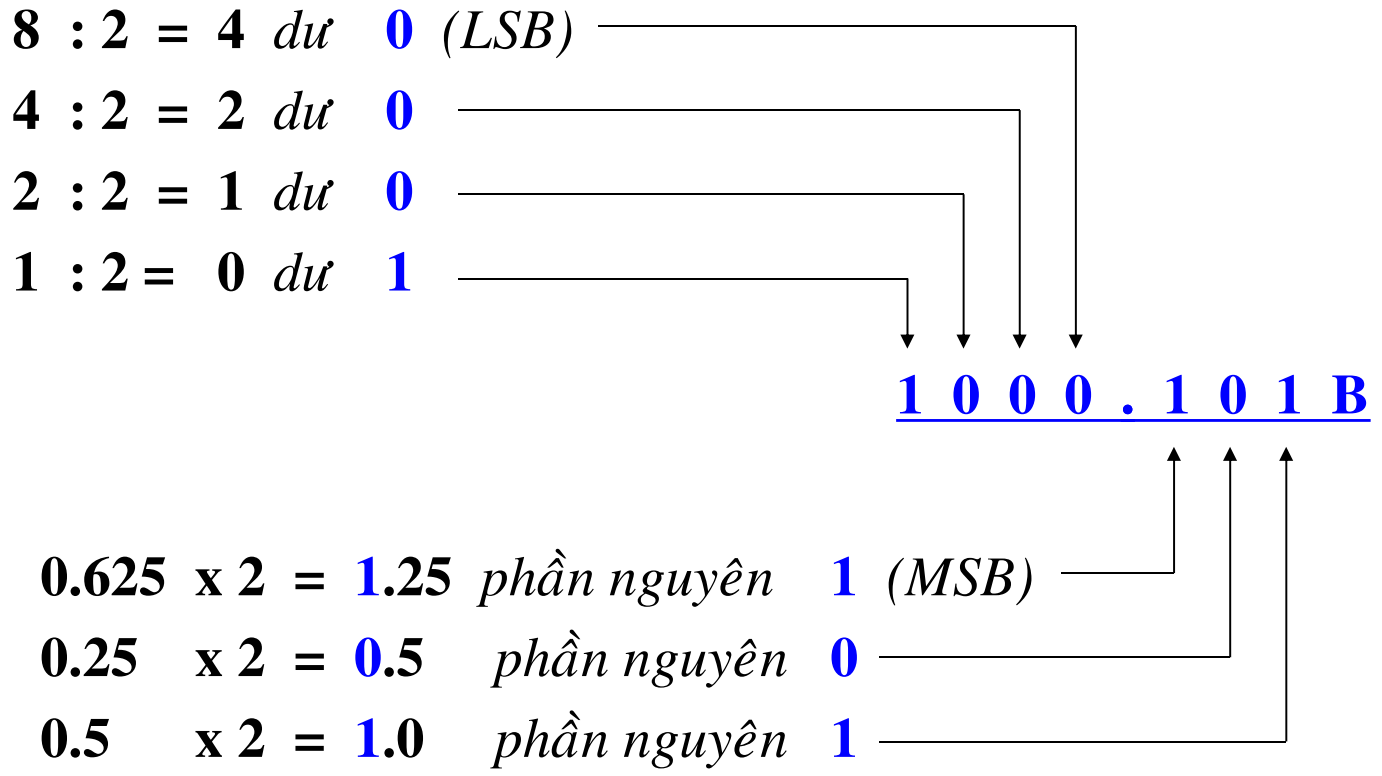
\includegraphics[width = 0.65\textwidth]{./local/image/1.png}
\end{center}
\textbf{b. Từ thập phân sang thập lục phân:}
\[
    1480.4296875
\]
\begin{center}
    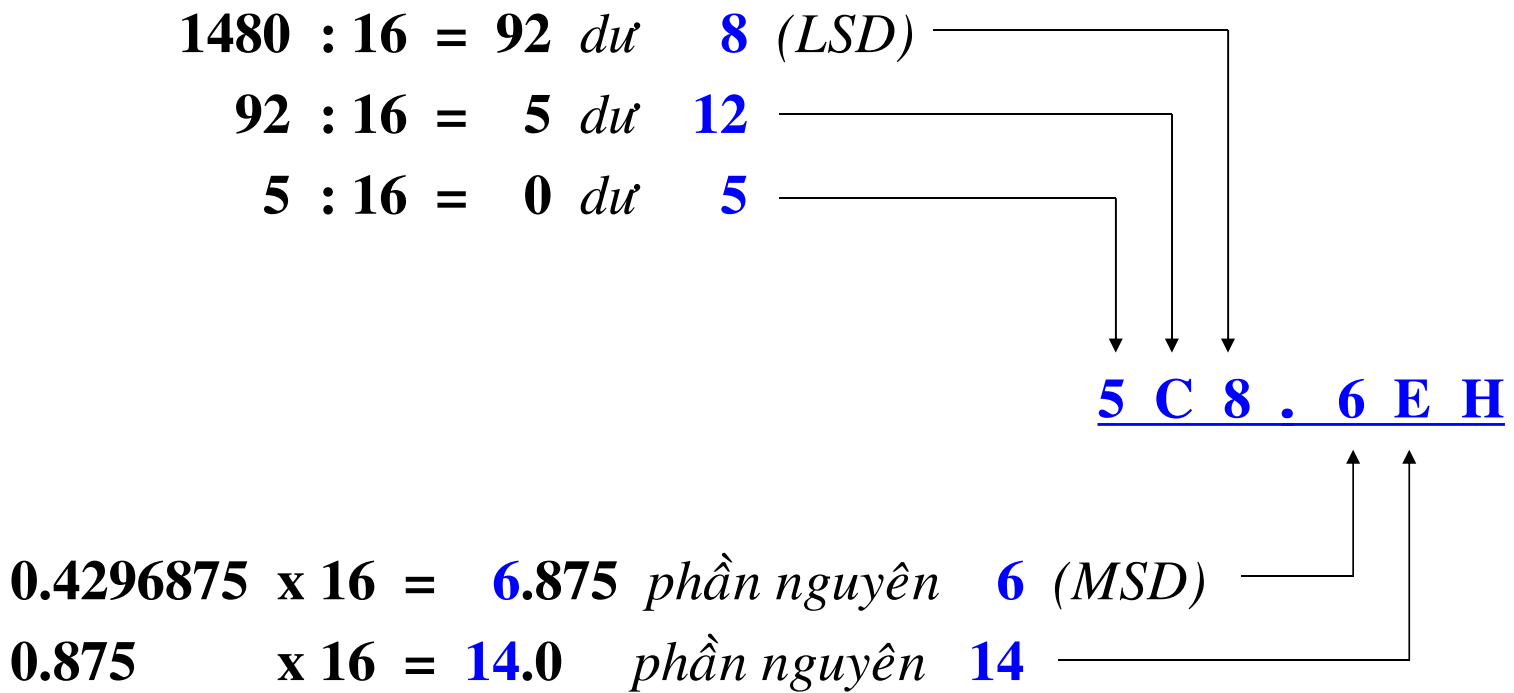
\includegraphics[width = 0.65\textwidth]{./local/image/2.png}
\end{center}
\textbf{c. Từ nhị phân sang thập lục phân}
\begin{center}
    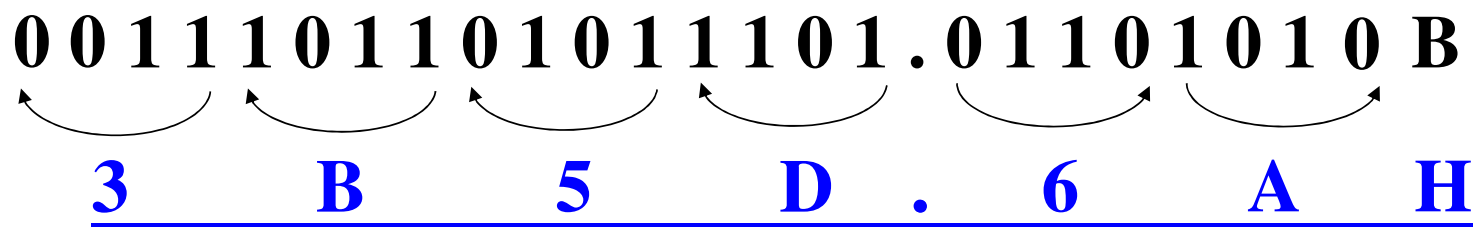
\includegraphics[width = 0.65\textwidth]{./local/image/3.png}
\end{center}
\textbf{d. Từ thập lục phân sang nhị phân}
\begin{center}
    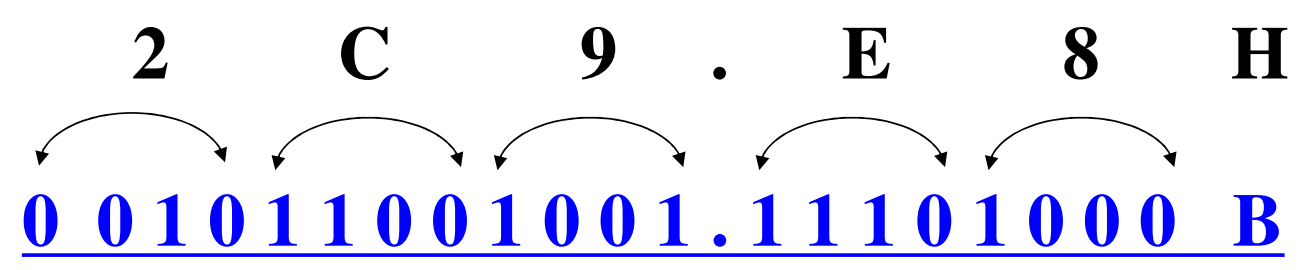
\includegraphics[width = 0.65\textwidth]{./local/image/4.png}
\end{center}
\section{Số nhị phân (Binary):}
\subsection{Các tính chất của số nhị phân}
\begin{itemize}
    \item[-] Số nhị phân n bit có $2^n$ giá trị từ $0$ đến $2^n-1$.
    \item[-] Số nhị phân có giá trị $2^n-1$: $1\cdots \cdots \cdots 1$ (n bit 1) và giá trị $2^n$: $1 \ 0 \cdots \cdots \cdots 0$ (n bit 0).
    \item[-] Số nhị phân có giá trị lẻ là số có LSB = 1; ngược lại giá trị chẵn là số có LSB = 0.
    \item[-] Các bội số của bit:
\end{itemize}
\begin{center}
    1 B (Byte) = 8 bit \\
    1 KB = $2^{10}$ B \\
    1 MB = $2^{10}$ KB \\
    1 GB = $2^{10}$ MB 
\end{center}
\subsection{Các phép toán số học trên số nhị phân:}
\noindent\textbf{a. Phép cộng}
\begin{center}
    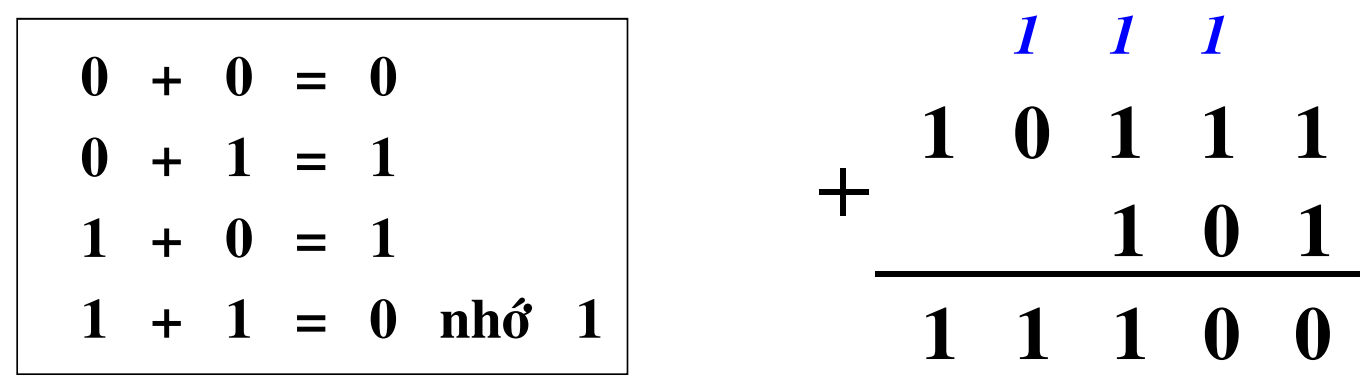
\includegraphics[width = 0.65\textwidth]{./local/image/5.png}
\end{center}
\textbf{b. Phép trừ}
\begin{center}
    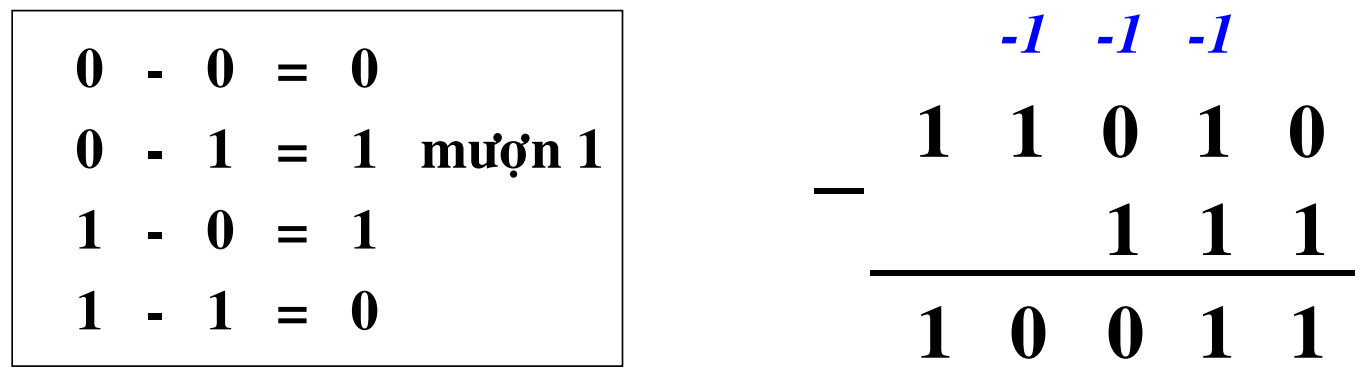
\includegraphics[width = 0.65\textwidth]{./local/image/6.png}
\end{center}
\textbf{c. Phép nhân}
\begin{center}
    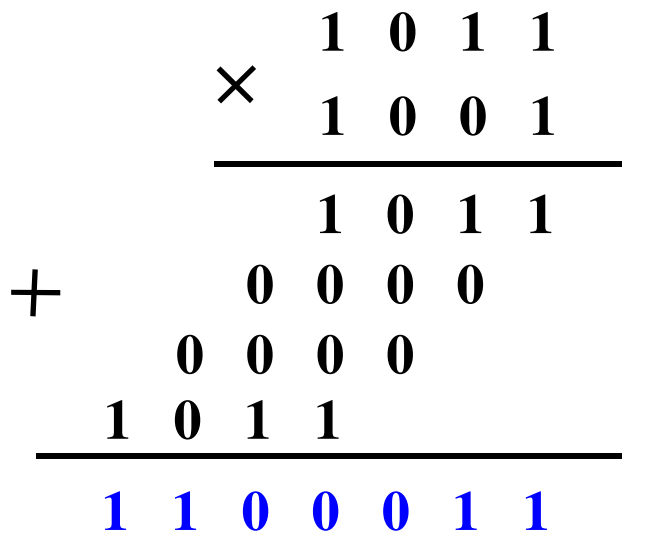
\includegraphics[width = 0.35\textwidth]{./local/image/7.png}
\end{center}
\textbf{d. Phép chia}
\begin{center}
    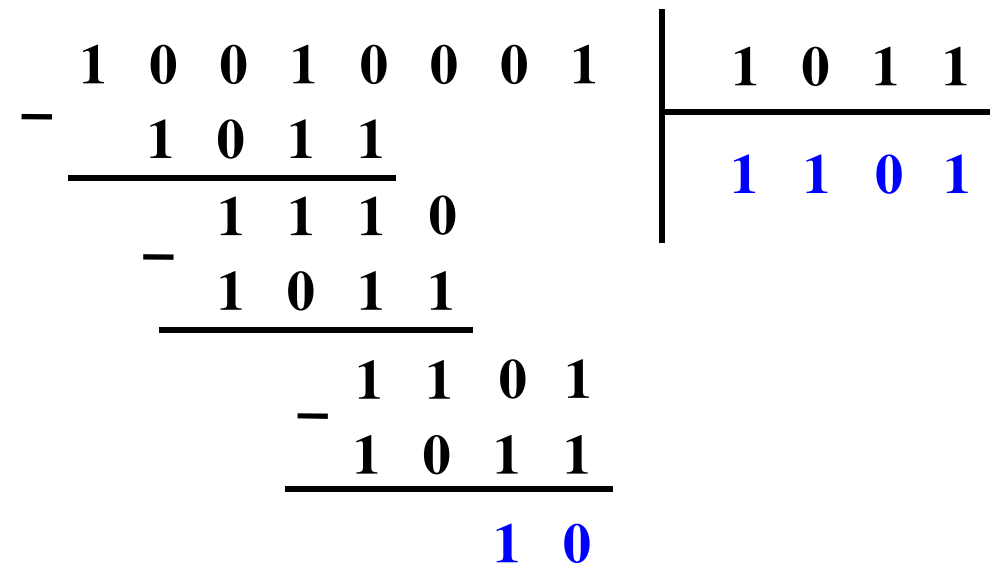
\includegraphics[width = 0.45\textwidth]{./local/image/8.png}
\end{center}
\subsection{Mã nhị phân:}
\textit{\textbf{Từ mã:}} là các tổ hợp nhị phân được sử dụng trong loại mã nhị phân.\\
\textbf{a. Mã nhị phân cho số thập phân (BCD - Binary Coded Decimal)}